\chapter*{Реферат}
\addcontentsline{toc}{chapter}{Реферат} %%To manually add unnumbered section, use the command \addcontentsline.

\begin{center}
    Общая характеристика диссертации
\end{center}

\paragraph*{Актуальность.}

\paragraph*{Цель исследования.}
\paragraph*{Научные задачи.}

\paragraph*{Методы исследования.}

\paragraph*{Основные положения, выносимые на защиту.}


\paragraph*{Научная новизна.}

\paragraph*{Теоретическая значимость.}
\paragraph*{Практическая значимость.}
\paragraph*{Достоверность.}
\paragraph*{Аппробация работы.}
Основные результаты диссертации докладывались на следующих конференциях:
\printConferenceRU

\paragraph*{Личный вклад автора.}


\paragraph*{Объём и структура работы.}
Диссертация состоит из введения,
\formbytotal{totalchapter}{глав}{ы}{}{},
заключения и
\formbytotal{totalappendix}{приложен}{ия}{ий}{}.
%% на случай ошибок оставляю исходный кусок на месте, закомментированным
%Полный объём диссертации составляет  \ref*{TotPages}~страницу
%с~\totalfigures{}~рисунками и~\totaltables{}~таблицами. Список литературы
%содержит \total{citenum}~наименований.
%
Полный объём диссертации составляет
\formbytotal{TotPages}{страниц}{у}{ы}{}, включая
\formbytotal{totalcount@figure}{рисун}{ок}{ка}{ков} и
\formbytotal{totalcount@table}{таблиц}{у}{ы}{}.
Список литературы содержит
\formbytotal{citenum}{наименован}{ие}{ия}{ий}.


\newpage
\section*{Основное содержание работы}

В Главе~\ref{ch:ch1}...

\begin{figure}
	\centering
	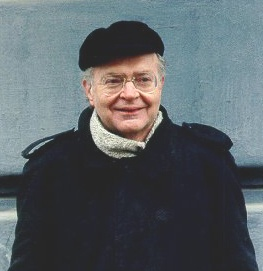
\includegraphics[width=0.4\linewidth]{images/knuth}
	\caption{Knuth}
	%\label{fig:my_label2}
\end{figure}

\begin{table}
	\centering
	\caption{Basic SI quantities}%\label{tab:unit:base}
	\begin{tabular}{llc}
		\toprule
		Name 	& 	Command 	& 	Symbol         \\
		\midrule
		Ampere     & \verb|\ampere| & \si{\ampere}   \\
		Candela   & \verb|\candela| & \si{\candela}  \\
		\bottomrule
	\end{tabular}
\end{table}

\begin{align} %\label{eq:sec1}
	1+2=3
\end{align}

\begin{assumption-syn-ru}
	Здесь и далее знак коэффициента при управлении $b_m$
	принимается известным. Без потери общности полагается $b_m >0$.
\end{assumption-syn-ru}
\begin{lemma-syn-ru} \label{lemma1}
	content...
\end{lemma-syn-ru}

\begin{proof}[Доказательство леммы \ref{lemma1}]
	content...
\end{proof}

\section*{Публикации автора по теме диссертации}

Основные результаты по теме диссертации изложены в \theAllMyPapers~публикациях. 
Из них \theScopusPapers~опубликовано в изданиях, индексируемых в базе цитирования Scopus, 
из них \theVakPapers~изданы в журналах, рекомендованных ВАК. 
%%Также имеется 1 свидетельство о государственной регистрации программ для ЭВМ.
%

В международных изданиях, индексируемых в базе данных Scopus, Web of Science:
\printPapperScopus

В изданиях из перечня ВАК РФ:
%\printPapperVak

В иных изданиях:
\printPapperOther
